\section{Deep Reinforcement Learning}
\subsection{Deep Value Function Approximation \& Automatic Differentiation}
In high-dimensional or continuous state spaces, linear value function approximation is insufficient to capture complex, non-linear relationships. Instead, Deep Neural Networks (DNNs) are used to parameterize value functions $v(s, \mathbf{w})$ or action-value functions $q(s, a, \mathbf{w})$.

\paragraph{Parameterization via Deep Networks.} A Multi-Layer Perceptron (MLP) calculates state values through sequential non-linear transformations:
$$v(S, \mathbf{w}) = \mathbf{W}_2 \tanh(\mathbf{W}_1 \cdot S + \mathbf{b}_1) + \mathbf{b}_2$$

where $\mathbf{w} = \{\mathbf{W}_1, \mathbf{b}_1, \mathbf{W}_2, \mathbf{b}_2\}$ represents the trainable weights and biases of the network.

\paragraph{Computational Graphs and Automatic Differentiation} Unlike linear function approximation (where gradients $\nabla_\mathbf{w} v(\cdot, \mathbf{w})$ are trivial to compute), deep architectures rely on computational graphs:
\begin{itemize}
    \item Computational Graph: Defines the sequence of operations as a Directed Acyclic Graph (DAG).
    \item Automatic Differentiation (Autodiff): Computes gradients of any output node with respect to any input parameter in a single backward sweep by applying the chain rule, accumulating products along paths, and summing gradients where paths merge.
\end{itemize}

\subsection{Deep Q-Learning (DQN)}
Deep Q-Learning parameterizes the action-value function $q_\mathbf{w}: \mathcal{S} \to \mathbb{R}^m$, mapping an input state $S_t$ to a vector of Q-values across $m$ discrete actions. 

\paragraph{Stabilizing Bootstrapping: Target Networks \& Experience Replay}
Standard Q-learning updates parameter vector $\mathbf{w}$ toward a bootstrapped target $Y_t = R_{t+1} + \gamma \max_{a} q(S_{t+1}, a, \mathbf{w})$. However, using the same weights $\mathbf{w}$ to compute both the prediction and the target causes severe instability: updating $\mathbf{w}$ to increase $q(S_t, A_t, \mathbf{w})$ simultaneously alters the target values for neighboring states, creating a moving target problem.

To resolve this, Deep Q-Networks (DQN) maintain two distinct networks:
\begin{enumerate}
    \item \textbf{Online Network ($q_\mathbf{w}$):} active parameters $\mathbf{w}$ that are continuously updated via gradient descent to select and evaluate actions.
    \item \textbf{Target Network ($q_{\mathbf{w}^-}$):} a semi-static copy with parameters $\mathbf{w}^-$, used exclusively to generate target labels $Y_t$. These parameters are periodically synchronized ($\mathbf{w}^- \leftarrow \mathbf{w}$) or softly updated every $C$ steps.
\end{enumerate}

Additionally, transitions $(S_t, A_t, R_{t+1}, S_{t+1})$ are stored in a replay buffer $\mathcal{D}$. Mini-batches of transitions are sampled uniformly to break temporal correlations between consecutive observations during optimization.

\paragraph{Loss Formulation}
The parameter update is framed as minimizing a Mean Squared Error (MSE) pseudo-loss over mini-batches sampled from $\mathcal{D}$:

$$L(\mathbf{w}) = \mathbb{E}_{(S_t, A_t, R_{t+1}, S_{t+1}) \sim \mathcal{D}} \left[ \frac{1}{2} \left( Y_t - q(S_t, A_t, \mathbf{w}) \right)^2 \right]$$

$$\text{where } Y_t = R_{t+1} + \gamma \max_{a} q\left(S_{t+1}, a, \mathbf{w}^-\right)$$

Because $Y_t$ is generated by the frozen target parameters $\mathbf{w}^-$, it acts as a fixed regression target during the update step. In automatic differentiation frameworks (e.g., JAX or PyTorch), this fixed-target treatment is enforced either by utilizing dedicated target network parameters or by applying a stop-gradient operator (\texttt{jax.lax.stop\_gradient}). Differentiating $L(\mathbf{w})$ with respect to $\mathbf{w}$ yields the desired semi-gradient update:

$$\nabla_{\mathbf{w}} L(\mathbf{w}) = - \mathbb{E}_{\mathcal{D}} \left[ \left( Y_t - q(S_t, A_t, \mathbf{w}) \right) \nabla_{\mathbf{w}} q(S_t, A_t, \mathbf{w}) \right]$$

\begin{figure}[htbp]
    \centering
    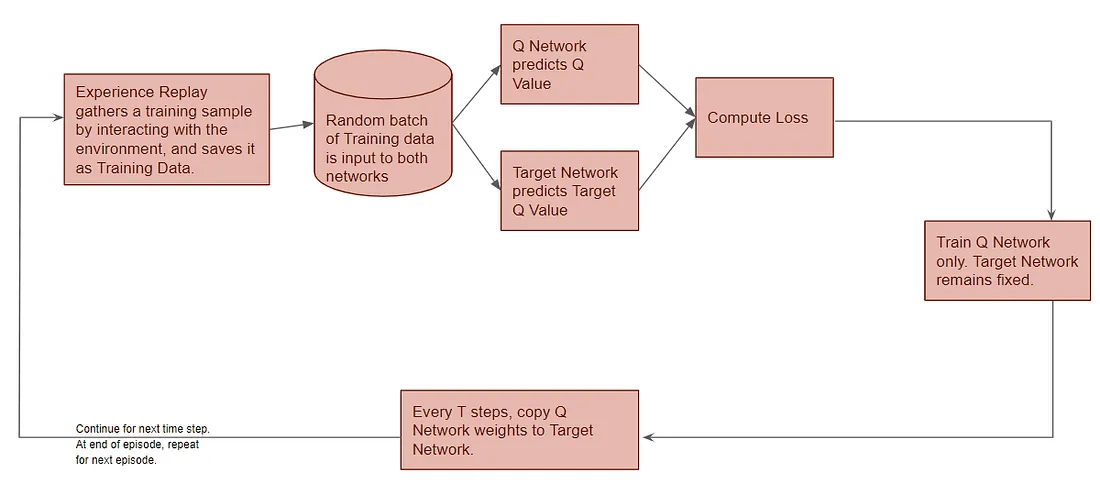
\includegraphics[width=0.70\textwidth]{figures/deep_q_learning.png}
\end{figure}

\subsection{Online Deep RL Issues \& Experience Replay}
Standard Deep Learning SGD optimization relies on the assumption that training data samples are independent and identically distributed (i.i.d.). Standard online RL violates this assumption:

\begin{itemize}
    \item \textbf{Online RL Bottleneck:} updates are performed on every step of sequential trajectories, resulting in highly correlated consecutive samples.
    \item \textbf{Experience Replay Solution:} stores historical transitions $(S_t, A_t, R_{t+1}, S_{t+1})$ in a buffer. Sampling mini-batches uniformly from the buffer:
    \begin{enumerate}
        \item Reduces correlation between consecutive updates.
        \item Enables stable mini-batch SGD updates instead of single-sample SGD.
    \end{enumerate}
    \item \textbf{Alternative Online Solutions:} Eligibility traces, momentum-based optimizers, and parallel environment execution.
\end{itemize}

\subsection{The Deadly Triad in Deep RL}
The Deadly Triad refers to the severe risk of divergence and instability arising when combining three core components:
\begin{enumerate}
    \item \textbf{Function Approximation:} fitting action values via neural networks
    \item \textbf{Bootstrapping:} target evaluation relying on estimated values
    \item \textbf{Off-Policy Learning:} learning from data collected under past/mixed policies
\end{enumerate}

\paragraph{Soft-Divergence}
In practical Deep RL settings, unbounded divergence is rare. Instead, algorithms suffer from soft-divergence -- transient value explosions that eventually recover after long training periods, severely degrading learning performance.

\subsection{RL-Aware Deep Learning Architectures \& Dynamics}
Rather than copying supervised learning architectures (e.g., standard CNNs/LSTMs), Deep RL benefits from structural inductive biases specifically designed for reinforcement learning dynamics.

\paragraph{Dueling Network Architecture} Decomposes action-value estimation into state-value and advantage streams:

$$q(s, a, \mathbf{w}) = v_\xi(s) + A_\chi(s, a) \quad \text{where } \mathbf{w} = \xi \cup \chi$$
\begin{itemize}
    \item $v_\xi(s)$: Represents how good it is to be in state $s$.
    \item $A_\chi(s, a)$: Represents the relative advantage of taking action $a$ over other actions.
\end{itemize}

\begin{figure}
    \centering
    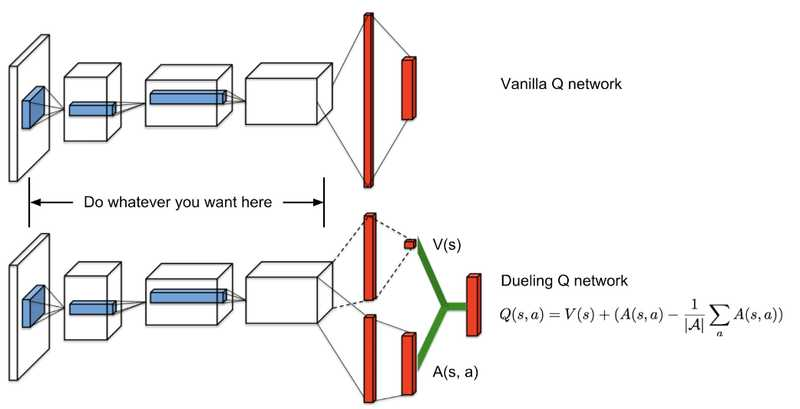
\includegraphics[width=0.65\textwidth]{figures/dueling-network-architectures.jpeg}
    \caption{Comparison between a standard DQN architecture (top) and a Dueling Q-network architecture (bottom). Both networks share identical convolutional feature-extraction layers. While vanilla DQN directly outputs action values $Q(s,a)$ from a single fully connected layer, the Dueling architecture splits into two separate streams to estimate state value $V(s)$ and action advantages $A(s,a)$, combining them via $Q(s,a) = V(s) + \left( A(s,a) - \frac{1}{|\mathcal{A}|}\sum_{a'} A(s,a') \right)$.}
    \label{fig:dueling_architecture}
\end{figure}

\textbf{Network Capacity \& Generalization Challenges}

\begin{itemize}
    \item \textbf{Capacity vs. Stability:} while increasing network size in supervised learning generally improves performance, larger networks in Deep RL are more susceptible to deadly triad instabilities despite achieving better final capacity.
    \item \textbf{Leakage Propagation:} combining Temporal Difference (TD) learning with deep function approximation leads to "leakage propagation," where approximation errors near sharp state-value discontinuities bleed into distant state regions. Monte Carlo methods do not suffer from leakage propagation.
    \item \textbf{Auxiliary Representation Learning:} to build representations resilient to improper generalization, state representations can be shared across auxiliary tasks—such as predicting values of multiple policies, predicting future observation frames, or controlling distinct auxiliary rewards (cumulants).
\end{itemize}
